\chapter{Các thuật toán Supervised Learning}

% ==========================================
% SECTION 1: TỔNG QUAN
% ==========================================
\section{Phân loại thuật toán Supervised Learning}

\begin{itemize}
    \item \textbf{Regression (Hồi quy):}
    \begin{itemize}
        \item Linear Regression (Hồi quy tuyến tính)
        \item Polynomial Regression (Hồi quy đa thức)
    \end{itemize}
    \item \textbf{Classification (Phân loại):}
    \begin{itemize}
        \item Logistic Regression
        \item Support Vector Machine (SVM)
        \item K-Nearest Neighbors (KNN)
        \item Naive Bayes
        \item Decision Tree
        \item Random Forest
    \end{itemize}
    \item $\rightarrow$ \textbf{Lưu ý về Naive Bayes:} Giả định các cột dữ liệu (feature) hoàn toàn độc lập với nhau (khó xảy ra trong thực tế vì các cột dữ liệu thường có mối quan hệ với nhau).
\end{itemize}

% ==========================================
% SECTION 2: LINEAR REGRESSION
% ==========================================
\section{Linear Regression (Hồi quy tuyến tính)}

\begin{figure}[H]
    \centering
    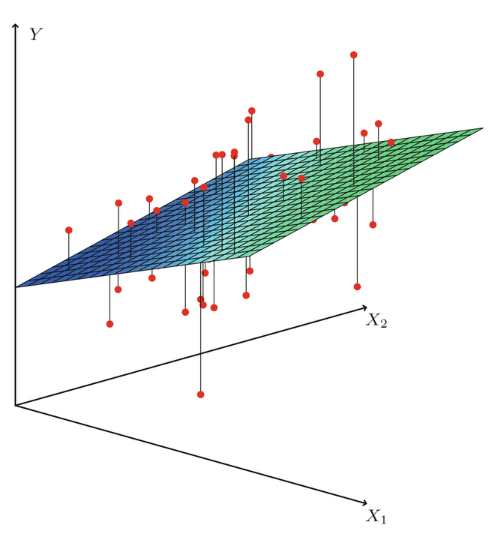
\includegraphics[width=0.8\linewidth]{21.png}
    %\fbox{\parbox[c][4cm][c]{0.8\linewidth}{\centering \textit{[Chèn ảnh: Minh họa Linear Regression tại đây]}}}
    \caption{Minh họa mô hình Linear Regression}
    \label{fig:linear_reg}
\end{figure}

\begin{itemize}
    \item Tìm đường thẳng tốt nhất sao cho tổng khoảng cách từ các điểm dữ liệu đến đường thẳng đó là bé nhất. Khi mở rộng ra không gian $n$ chiều ($n > 3$), đường thẳng trở thành \textbf{siêu phẳng (hyperplane)}.
    \item Là mô hình bậc 1.
    \item Phù hợp với dataset tuyến tính, có mối quan hệ tuyến tính giữa feature và target.
    \item Biểu diễn dạng vector: $\mathbf{x} = [x_1, x_2, x_3]^T$ là vector đầu vào (input).
    \item Tìm nghiệm để tối ưu hàm mất mát $L$.
    \item \textbf{Hạn chế của Linear Regression:}
    \begin{itemize}
        \item Nhạy cảm với nhiễu (outlier).
        \item Không biểu diễn được các mô hình phức tạp.
    \end{itemize}
\end{itemize}

% ==========================================
% SECTION 3: POLYNOMIAL REGRESSION
% ==========================================
\section{Polynomial Regression (Hồi quy đa thức)}

\begin{figure}[H]
    \centering
    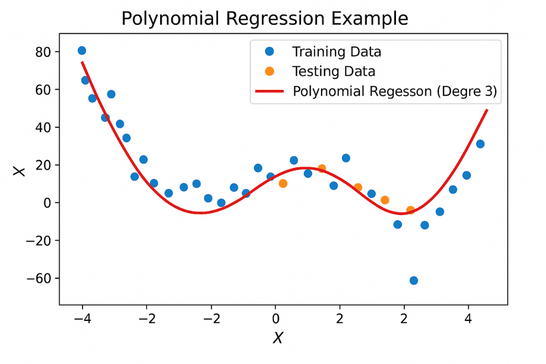
\includegraphics[width=0.8\linewidth]{22.png}
    %\fbox{\parbox[c][4cm][c]{0.8\linewidth}{\centering \textit{[Chèn ảnh: Minh họa Polynomial Regression tại đây]}}}
    \caption{Minh họa mô hình Polynomial Regression}
    \label{fig:poly_reg}
\end{figure}

\begin{itemize}
    \item Là mô hình có bậc lớn hơn 1.
    \item Cho khả năng dự đoán tốt hơn trên dữ liệu phi tuyến tính, nhưng đồng thời cũng \textbf{dễ bị Overfitting} hơn.
\end{itemize}

% ==========================================
% SECTION 4: LOGISTIC REGRESSION
% ==========================================
\section{Logistic Regression}

\begin{figure}[H]
    \centering
    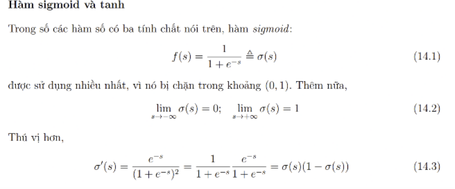
\includegraphics[width=0.8\linewidth]{23.png}
    %\fbox{\parbox[c][4cm][c]{0.8\linewidth}{\centering \textit{[Chèn ảnh: Hàm Sigmoid và Logistic Regression tại đây]}}}
    \caption{Hàm Sigmoid trong Logistic Regression}
    \label{fig:logistic_reg}
\end{figure}

\begin{itemize}
    \item Sử dụng \textbf{hàm Sigmoid} để chuyển đầu ra (output) về thang đo $[0, 1]$.
    \item Chia đoạn để phân lớp, ví dụ: $[0, 0.5] \rightarrow \text{Class 1}$, $(0.5, 1] \rightarrow \text{Class 2}$.
    \item \textbf{Threshold (Ngưỡng):} Điểm phân định ranh giới, điểm kích hoạt để chuyển đổi từ trạng thái (class) này sang trạng thái khác.
\end{itemize}
\begin{figure}[H]
    \centering
    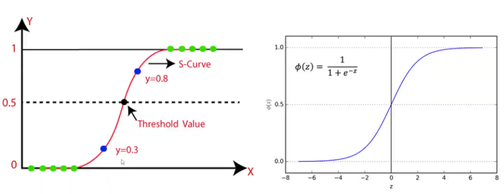
\includegraphics[width=0.8\linewidth]{24.png}
    %\fbox{\parbox[c][4cm][c]{0.8\linewidth}{\centering \textit{[Chèn ảnh: Hàm Sigmoid và Logistic Regression tại đây]}}}
    \caption{Hàm Sigmoid trong Logistic Regression}
    \label{fig:logistic_reg2}
\end{figure}

% ==========================================
% SECTION 5: SUPPORT VECTOR MACHINE (SVM)
% ==========================================
\section{Support Vector Machine (SVM)}

\begin{figure}[H]
    \centering
    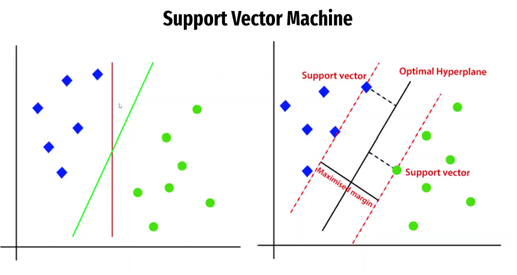
\includegraphics[width=0.8\linewidth]{25.png}
    %\fbox{\parbox[c][4cm][c]{0.8\linewidth}{\centering \textit{[Chèn ảnh: Minh họa Support Vector và Margin tại đây]}}}
    \caption{Nguyên lý hoạt động của Support Vector Machine}
    \label{fig:svm}
\end{figure}


\begin{itemize}
    \item Tập trung vào các điểm dữ liệu nằm trên ranh giới để phân định chúng, từ đó tạo ra đường/vector phân cách giữa các class. Thay vì fit toàn bộ các điểm dữ liệu, SVM chỉ xử lý các điểm dễ phân loại sai.
    \item \textbf{Support Vector:} Là những điểm dễ sai nhất vì chúng nằm sát đường phân cách.
    \item \textbf{Hai điều kiện để chọn đường phân cách tối ưu:}
    \begin{itemize}
        \item Khoảng cách từ hai điểm gần nhất của hai miền đến đường phân cách phải \textbf{bằng nhau}.
        \item Phải tạo ra được \textbf{khoảng cách (margin) tối đa} giữa Support Vector và đường phân cách.
    \end{itemize}
    \item $\rightarrow$ \textbf{Xử lý dữ liệu thực tế (Not Linearly Separable):}
    \begin{itemize}
        \item Khi dữ liệu không thể tách tuyến tính trong không gian hiện tại, SVM sẽ thêm chiều mới vào (chiều mới là tổ hợp của các chiều cũ $\rightarrow$ tạo thêm nhiều feature mới).
        \item Tiếp tục thêm chiều mới cho đến khi có thể phân chia được các lớp.
    \end{itemize}
\end{itemize}
\begin{figure}[H]
    \centering
    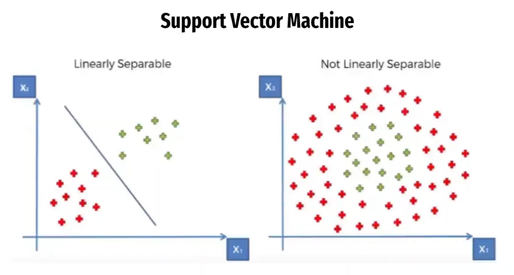
\includegraphics[width=0.8\linewidth]{26.png}
    %\fbox{\parbox[c][4cm][c]{0.8\linewidth}{\centering \textit{[Chèn ảnh: Minh họa Support Vector và Margin tại đây]}}}
    \caption{minh họa}
    \label{fig:svm1}
\end{figure}

\begin{figure}[H]
    \centering
    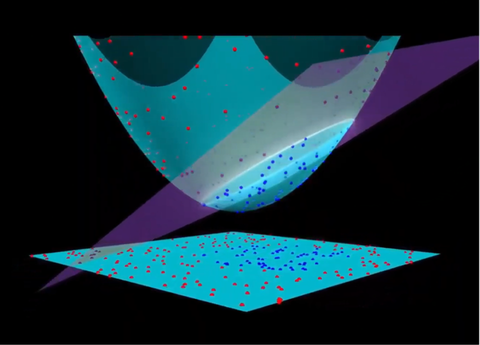
\includegraphics[width=0.8\linewidth]{27.png}
    %\fbox{\parbox[c][4cm][c]{0.8\linewidth}{\centering \textit{[Chèn ảnh: Minh họa Support Vector và Margin tại đây]}}}
    \caption{minh họa}
    \label{fig:svm2}
\end{figure}

\begin{figure}[H]
    \centering
    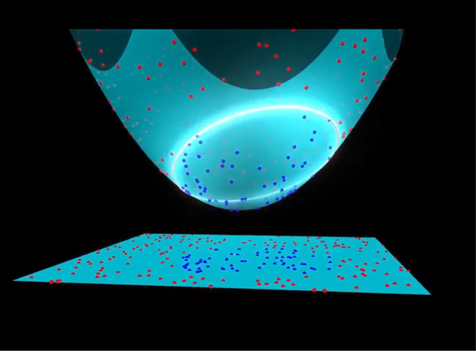
\includegraphics[width=0.8\linewidth]{28.png}
    %\fbox{\parbox[c][4cm][c]{0.8\linewidth}{\centering \textit{[Chèn ảnh: Minh họa Support Vector và Margin tại đây]}}}
    \caption{minh họa}
    \label{fig:svm3}
\end{figure}

\begin{figure}[H]
    \centering
    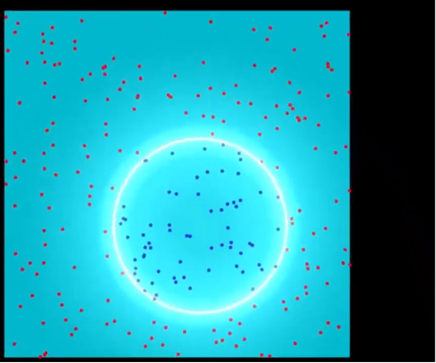
\includegraphics[width=0.8\linewidth]{29.png}
    %\fbox{\parbox[c][4cm][c]{0.8\linewidth}{\centering \textit{[Chèn ảnh: Minh họa Support Vector và Margin tại đây]}}}
    \caption{minh họa}
    \label{fig:svm4}
\end{figure}

\begin{figure}[H]
    \centering
    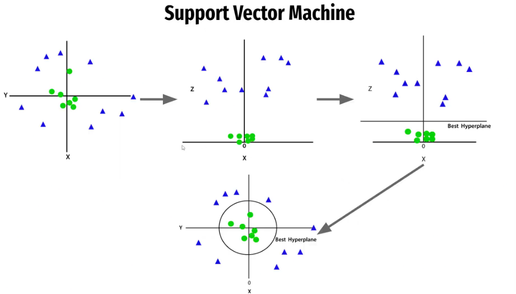
\includegraphics[width=0.8\linewidth]{30.png}
    %\fbox{\parbox[c][4cm][c]{0.8\linewidth}{\centering \textit{[Chèn ảnh: Minh họa Support Vector và Margin tại đây]}}}
    \caption{minh họa}
    \label{fig:svm5}
\end{figure}
% ==========================================
% SECTION 6: K-NEAREST NEIGHBORS (KNN)
% ==========================================
\section{K-Nearest Neighbors (KNN)}

\begin{figure}[H]
    \centering
    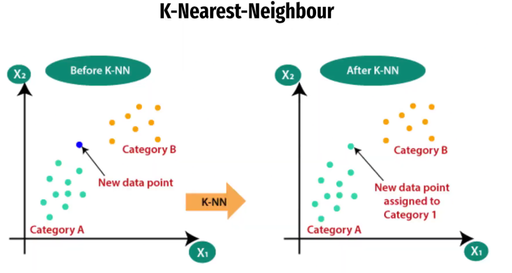
\includegraphics[width=0.8\linewidth]{31.png}
    %\fbox{\parbox[c][4cm][c]{0.8\linewidth}{\centering \textit{[Chèn ảnh: Minh họa thuật toán KNN tại đây]}}}
    \caption{Nguyên lý phân loại của K-Nearest Neighbors}
    \label{fig:knn}
\end{figure}

\begin{itemize}
    \item Khi có một điểm dữ liệu mới cần phân loại, thuật toán sẽ chọn ra $K$ điểm gần nó nhất rồi xét xem class nào chiếm đa số thì gán điểm mới vào class đó.
    \item \textbf{Tính khoảng cách:} Vì dựa vào độ gần, các feature bắt buộc phải được chuẩn hóa để phạm vi (range) của từng feature công bằng với nhau, tránh việc giá trị lớn của một feature áp đảo các feature khác.
    \item Thường chọn $K$ là \textbf{số lẻ} (để tránh hòa phiếu), không nên chọn $K$ quá bé hoặc quá lớn.
    \item \textbf{Đặc điểm:} Thời gian huấn luyện $\text{Training} = 0$; quá trình tính toán chỉ thực sự diễn ra lúc thực thi (dự đoán).
\end{itemize}

% ==========================================
% SECTION 7: DECISION TREE
% ==========================================
\section{Decision Tree (Cây quyết định)}

\begin{figure}[H]
    \centering
    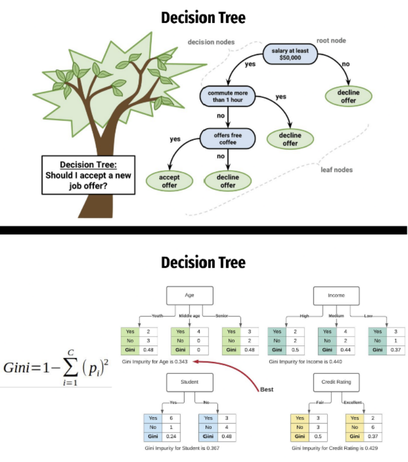
\includegraphics[width=0.8\linewidth]{32.png}
    %\fbox{\parbox[c][4cm][c]{0.8\linewidth}{\centering \textit{[Chèn ảnh: Cấu trúc Decision Tree tại đây]}}}
    \caption{Cấu trúc của một Decision Tree}
    \label{fig:decision_tree}
\end{figure}

\begin{itemize}
    \item \textbf{Các thành phần chính:}
    \begin{itemize}
        \item \textbf{Decision Nodes:} Các nút quyết định (nơi rẽ nhánh theo điều kiện).
        \item \textbf{Leaf Nodes:} Các nút lá (chứa kết quả phân loại/dự đoán cuối cùng).
    \end{itemize}
    \item \textbf{Gini Index (Gini Impurity):} Chỉ số dùng để tính toán và chọn feature làm nút gốc (root) cho các cây con. Giá trị càng gần $0$ càng tốt (thuần khiết), càng gần $0.5$ càng tồi (hỗn tạp).
    \item \textbf{Ưu điểm:}
    \begin{itemize}
        \item Có thể giải quyết tốt các bài toán phi tuyến tính.
        \item Làm việc với không gian nhiều chiều (nhiều feature) với độ chính xác cao.
        \item Rất trực quan và dễ dàng giải thích kết quả.
    \end{itemize}
\end{itemize}

% ==========================================
% SECTION 8: RANDOM FOREST
% ==========================================
\section{Random Forest}

\begin{figure}[H]
    \centering
    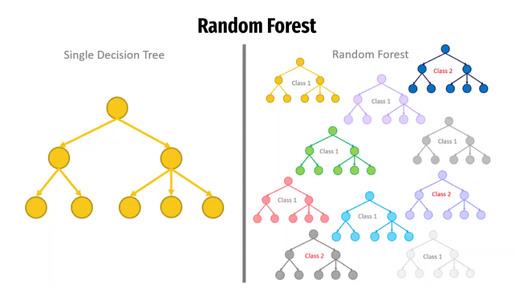
\includegraphics[width=0.8\linewidth]{33.png}
    %\fbox{\parbox[c][4cm][c]{0.8\linewidth}{\centering \textit{[Chèn ảnh: Mô hình Random Forest tại đây]}}}
    \caption{Cơ chế kết hợp nhiều cây trong Random Forest}
    \label{fig:random_forest}
\end{figure}
\begin{figure}[H]
    \centering
    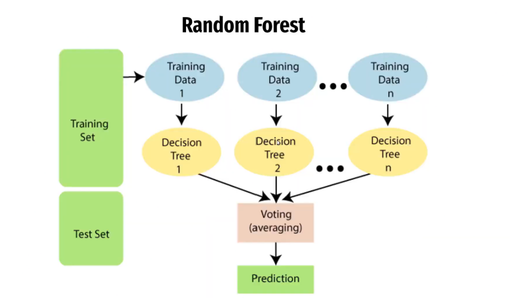
\includegraphics[width=0.8\linewidth]{34.png}
    %\fbox{\parbox[c][4cm][c]{0.8\linewidth}{\centering \textit{[Chèn ảnh: Mô hình Random Forest tại đây]}}}
    \caption{Cơ chế kết hợp nhiều cây trong Random Forest}
    \label{fig:random_forest1}
\end{figure}

\begin{itemize}
    \item Không huấn luyện toàn bộ các cây trên toàn bộ tập dữ liệu, mà chia nhỏ bộ dataset và chọn ngẫu nhiên một tập con các feature cho từng cây.
    \item Cho độ tin cậy cao hơn và giảm overfitting tốt hơn so với một cây Decision Tree đơn lẻ.
\end{itemize}